%!TEX root = ../../super_main.tex

\section{Background Sensor Service}
\label{sec:background_sensor_service}

We have implemented a service, which we call Background Sensor Service, in order to facility non-intrusive data collection in the Android system.
This section includes some technical details about how services work in Android and how we have implemented our Background Sensor Service. 

\subsection{What is an Android service?}

A services in Android is an application component which encapsulates long running background processing or a way to provide access to a shared ressource. Services can be shared and can be configured run independently, i.e. running in a different process, from the graphical interface shown to users, which is ideal for our background data collection. Services have their own lifecycles and can be configured in many different ways. They can be configured as an API where the service itself has a short lifespan while serving some data or while performing a short task or they can be configured as a long running background task with its own complex behavior.
\\\\
% Message parsing
The Android framework supports two-way message parsing as a way of communication with a service when it runs in a different process. Message parsing makes it easy for the Android \mono{Activity} elements in the graphical and interactive part of the application to communicate with our Background Sensor Service.
\\\\
We have given an overview of the concurrency 

\subsection{Service Start}

% Boot receiver
% On Application start
Our Background Sensor Service should ideally always be running, which does not imply that it is constantly using processing ressources. We have implemented two measures to ensures that the service is running for as much time as possible. We have implemented an Android BroadcastReceiver, which upon receiving a system wide boot completed action (\mono{ACTION\_BOOT\_COMPLETED}), starts the service. The service is also attempted started everytime the application is started, but is not started twice if the service is already running. 

\subsection{Snapshot Generation and Synchronization}
\label{sub:background_sensor_service_snapshot_generation_and_synchronization}

The background Background Sensor Service uses two independent timers. One for snapshot generation and one for synchronization of the snapshots with our server. The timer for snapshot generation is encapsulated in a class called \mono{SnapshotTimer} which is started whenever the service has an active running campaign which should generate snapshots. Timed tasks are then scheduled at a constant rate, generating snapshots, until the campaign is completed or stopped by the user.
\\\\
Synchronization of snapshots with the server is done with the second timer which is encapsulated in a class called \mono{SynchronizationTimer}. This timer schedules tasks, when active, which attempts to synchronize gathered snapshots with the server at a fixed rate if the device is currently connected to a Wi-Fi network. This is not an optimal solution as it does not incorporate any battery consumption optimizations except maybe for a little bundling of the data in the given temporal frame until the next synchronization. The actual size of the bundled data is not taken into account so the bundling of the collected data is probably not that effective, especially not for data sets collected at a low frequency. The \mono{SynchronizationTimer} also does not incorporate any radio based optimizations such as scheduling network task through Android APIs. The \mono{SynchronizationTimer} just requests immediate communication over the Wi-Fi connection which forces waking up radio hardware if it was in a dormant state. This is not ideal as we do not require data to be uploaded as soon as its ready as stated in \todo{Byg ref til vores opsummering af krav jf. task til at gøre det} and because there is potential for less battery consumption which would help satisfy \todo{ref til konkret requirement }. 
\\\\
An example of an Android API, or rather a library with Google APIs for Android, which could help optimize network usage would be the \mono{GCMNetworkManager} class, which is an Android service, that can schedule encapsulated network tasks. \mono{GCMNetworkManager} \parencite{gcmnetworkmanager} handles batching of network tasks; retries; backoffs, in case a remote server is not responding or is busy; waiting for Wi-Fi, for bandwidth heavy communication; waiting with commutation until the device is charging; and waiting until a radio becomes active, for instance by getting activated by another application. It does all of this based on parameters given to every encapsulated network tasks such as a desired time frame for the network communication and desired network or battery conditions.  
\\\\
Adding such optimizations should however be doable as all data synchronization work is local to the \mono{SynchronizationTimer} and not distributed elsewhere in the implementation. Other network tasks such a refreshing GUI with lists of campaigns from the service should happen instantly and are thus more difficult to optimize. 

\subsection{Background Sensor Listening}

The Background Sensor Service is configured to have one thread, in a pool of threads, available per sensor type, i.e. per \mono{SensorProvider}, see \secref{sub:providing_sensor_data_implementation}, instance used in the service. This lets the scheduling of the gathering from the different \mono{SensorProvider} instances up to the underlying Java implementation of threads in a hope to run the different types of sensors and other data sources as independently as possible. Data is only collected from the \mono{SensorProvider} instances if the corresponding sensors are included in the currently active campaign and if the system is currently gathering a snapshot. There is no data collection activity in the Background Sensor Service unless a timed task for a snapshot is running. CPU resources and thereby battery is therefore only consumed on demand.
\\\\
We do not provide any real time guarantees but the different threads from the different streams of data should always be able to run unless they get starved by other processes in the system. Temporary starvation of the data collecting threads might result in missed updates from different data sources. 

\subsection{Concurrency Overview}

We have attempted to give an overview of the current processes and threads running in the mobile application in \figref{fig:system_currency_and_lifecycle} illustrated with a near UML Activity Diagram Syntax. 

\begin{figure}[!htbp]
    \centering
    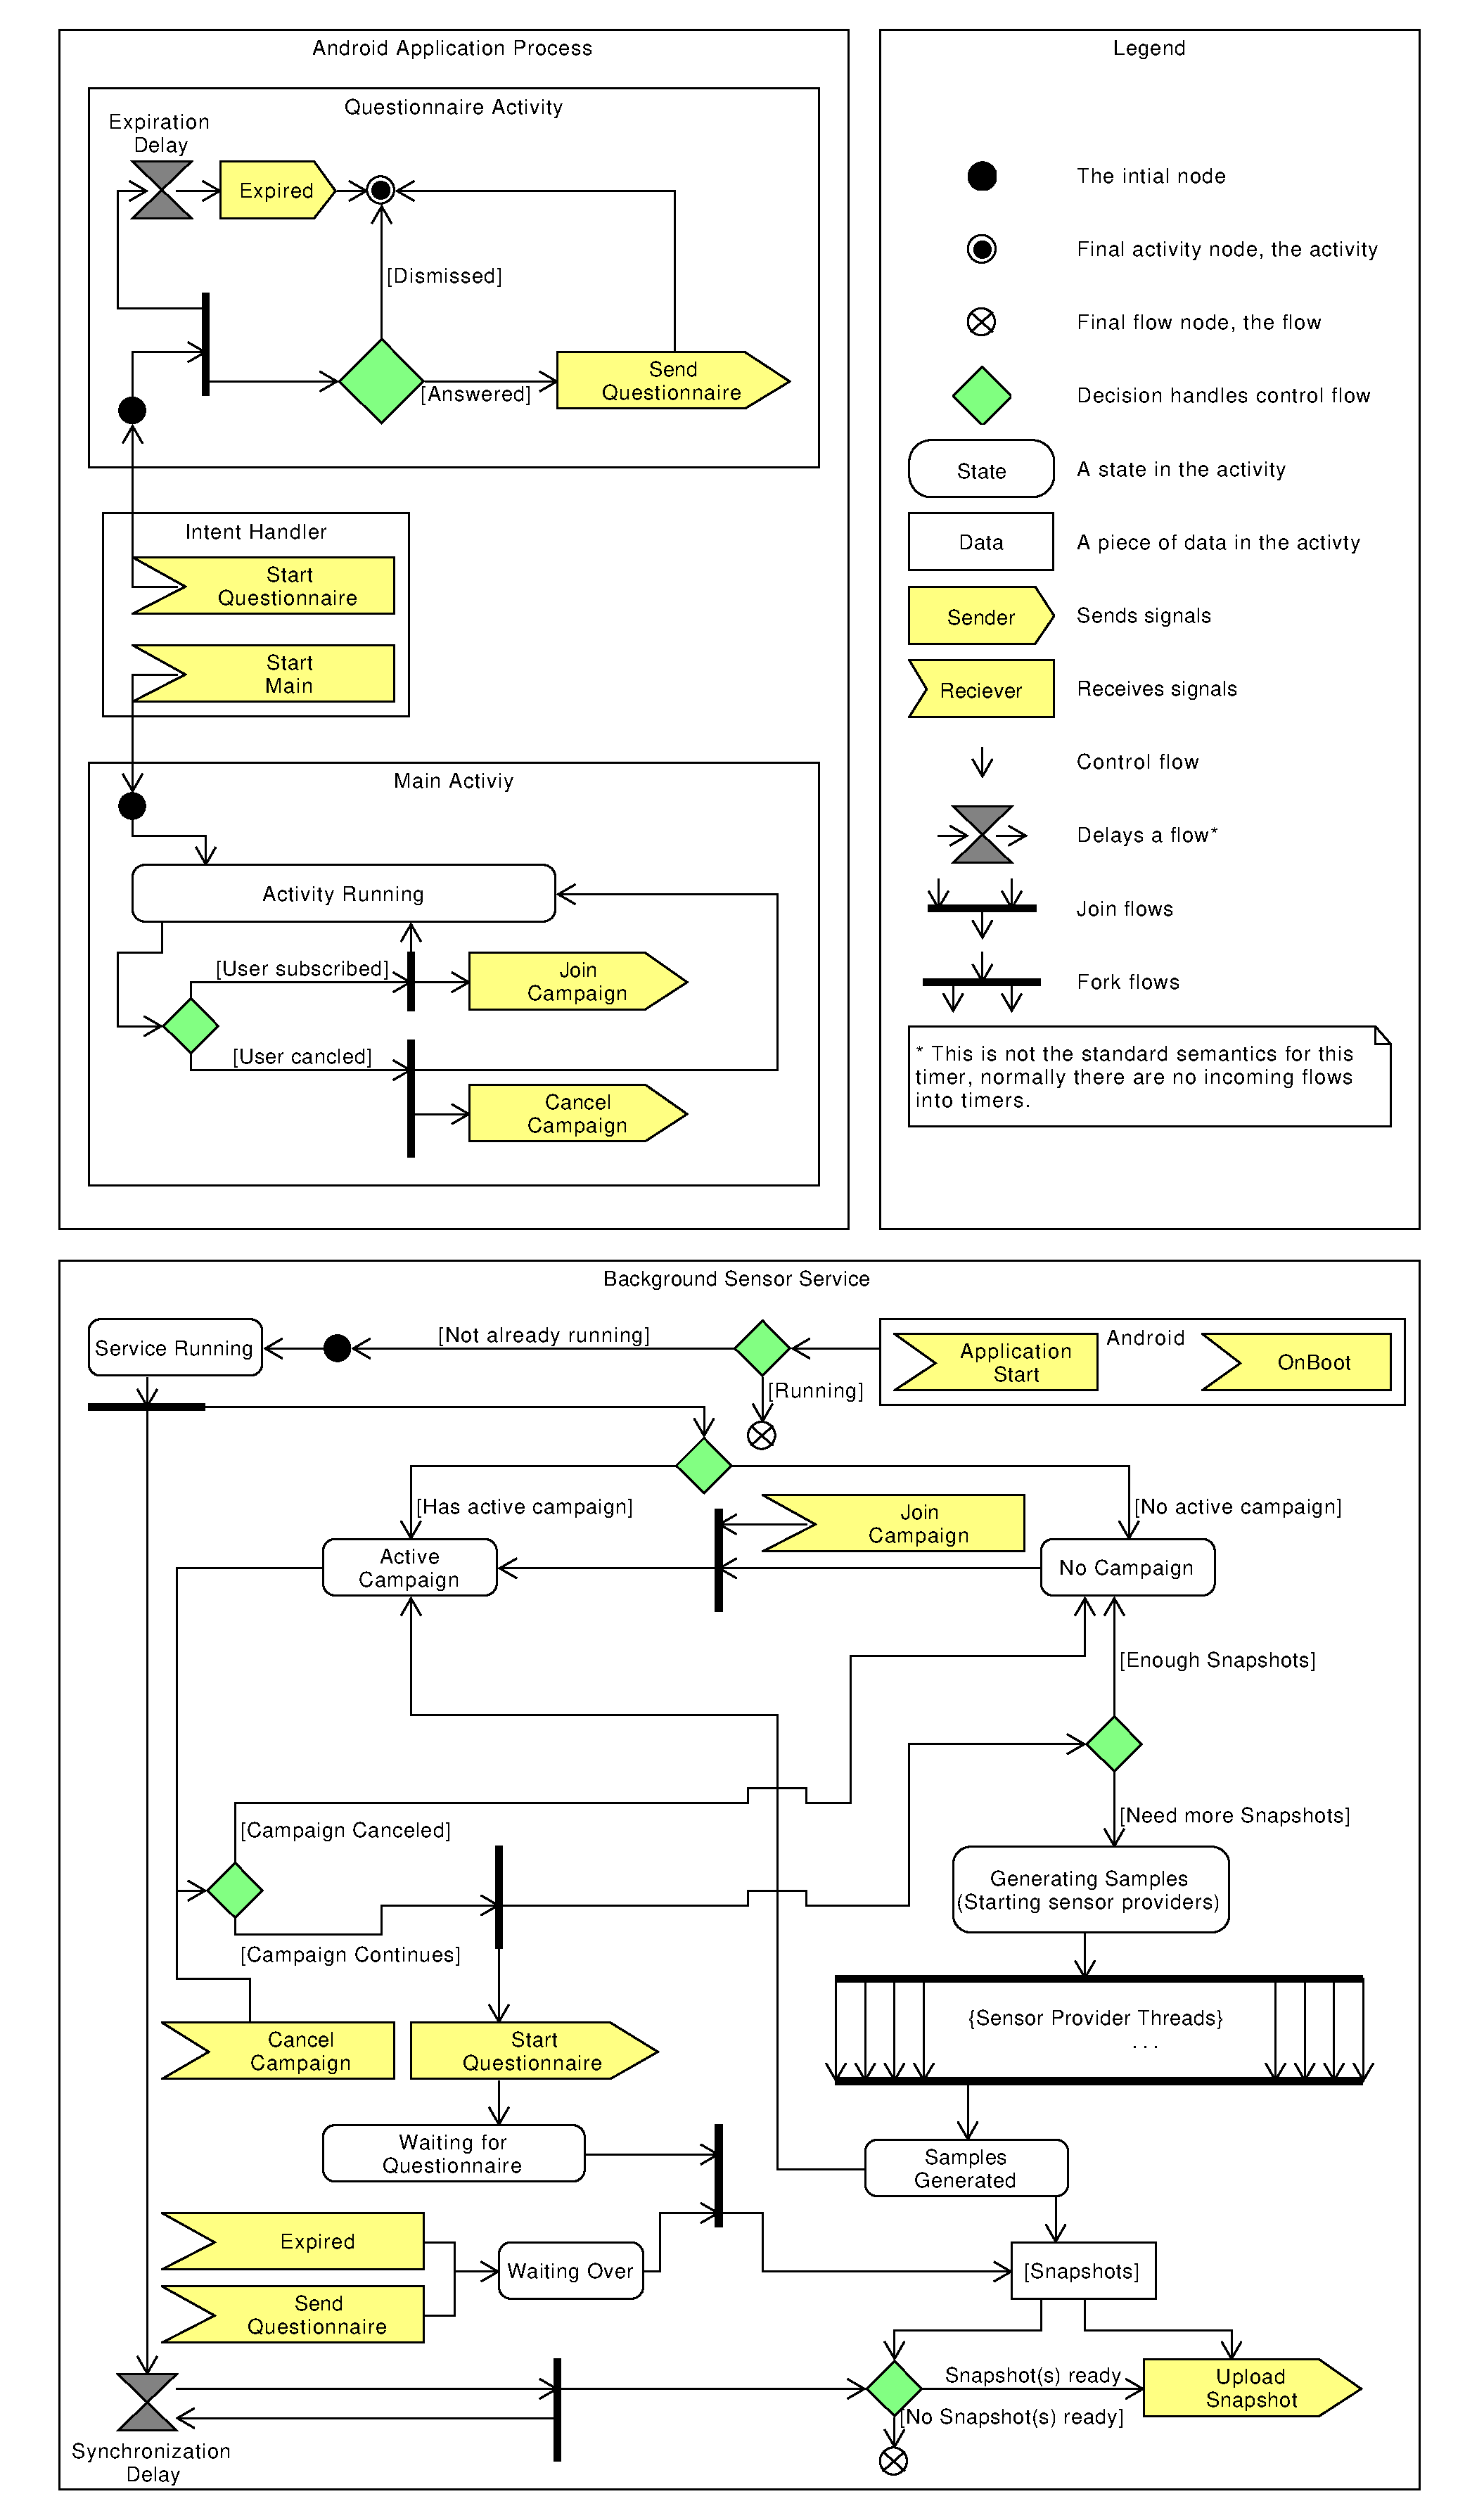
\includegraphics[width=\textwidth]{graphic/backgroundsensorservice/lifecyclestuff.pdf}
    \caption{An Activiy Diagram like overview of the mobile Application Components.}
    \label{fig:system_currency_and_lifecycle}
\end{figure}
\FloatBarrier